\documentclass{book}
\usepackage[a4paper,top=2.5cm,bottom=2.5cm,left=2.5cm,right=2.5cm]{geometry}
\usepackage{makeidx}
\usepackage{natbib}
\usepackage{graphicx}
\usepackage{multicol}
\usepackage{float}
\usepackage{listings}
\usepackage{color}
\usepackage{ifthen}
\usepackage[table]{xcolor}
\usepackage{textcomp}
\usepackage{alltt}
\usepackage{ifpdf}
\ifpdf
\usepackage[pdftex,
            pagebackref=true,
            colorlinks=true,
            linkcolor=blue,
            unicode
           ]{hyperref}
\else
\usepackage[ps2pdf,
            pagebackref=true,
            colorlinks=true,
            linkcolor=blue,
            unicode
           ]{hyperref}
\usepackage{pspicture}
\fi
\usepackage[utf8]{inputenc}
\usepackage{mathptmx}
\usepackage[scaled=.90]{helvet}
\usepackage{courier}
\usepackage{sectsty}
\usepackage[titles]{tocloft}
\usepackage{doxygen}
\lstset{language=C++,inputencoding=utf8,basicstyle=\footnotesize,breaklines=true,breakatwhitespace=true,tabsize=8,numbers=left }
\makeindex
\setcounter{tocdepth}{3}
\renewcommand{\footrulewidth}{0.4pt}
\renewcommand{\familydefault}{\sfdefault}
\hfuzz=15pt
\setlength{\emergencystretch}{15pt}
\hbadness=750
\tolerance=750
\begin{document}
\hypersetup{pageanchor=false,citecolor=blue}
\begin{titlepage}
\vspace*{7cm}
\begin{center}
{\Large My Project }\\
\vspace*{1cm}
{\large Generated by Doxygen 1.8.1}\\
\vspace*{0.5cm}
{\small Fri Jun 22 2012 15:11:43}\\
\end{center}
\end{titlepage}
\clearemptydoublepage
\pagenumbering{roman}
\tableofcontents
\clearemptydoublepage
\pagenumbering{arabic}
\hypersetup{pageanchor=true,citecolor=blue}
\chapter{Class Index}
\section{Class Hierarchy}
This inheritance list is sorted roughly, but not completely, alphabetically\-:\begin{DoxyCompactList}
\item \contentsline{section}{A\-P\-Keypad}{\pageref{class_a_p_keypad}}{}
\begin{DoxyCompactList}
\item \contentsline{section}{A\-P\-Numpad}{\pageref{class_a_p_numpad}}{}
\end{DoxyCompactList}
\end{DoxyCompactList}

\chapter{Class Index}
\section{Class List}
Here are the classes, structs, unions and interfaces with brief descriptions\-:\begin{DoxyCompactList}
\item\contentsline{section}{\hyperlink{class_a_p_keypad}{A\-P\-Keypad} }{\pageref{class_a_p_keypad}}{}
\item\contentsline{section}{\hyperlink{class_a_p_numpad}{A\-P\-Numpad} }{\pageref{class_a_p_numpad}}{}
\end{DoxyCompactList}

\chapter{Class Documentation}
\hypertarget{class_a_p_keypad}{\section{A\-P\-Keypad Class Reference}
\label{class_a_p_keypad}\index{A\-P\-Keypad@{A\-P\-Keypad}}
}
Inheritance diagram for A\-P\-Keypad\-:\begin{figure}[H]
\begin{center}
\leavevmode
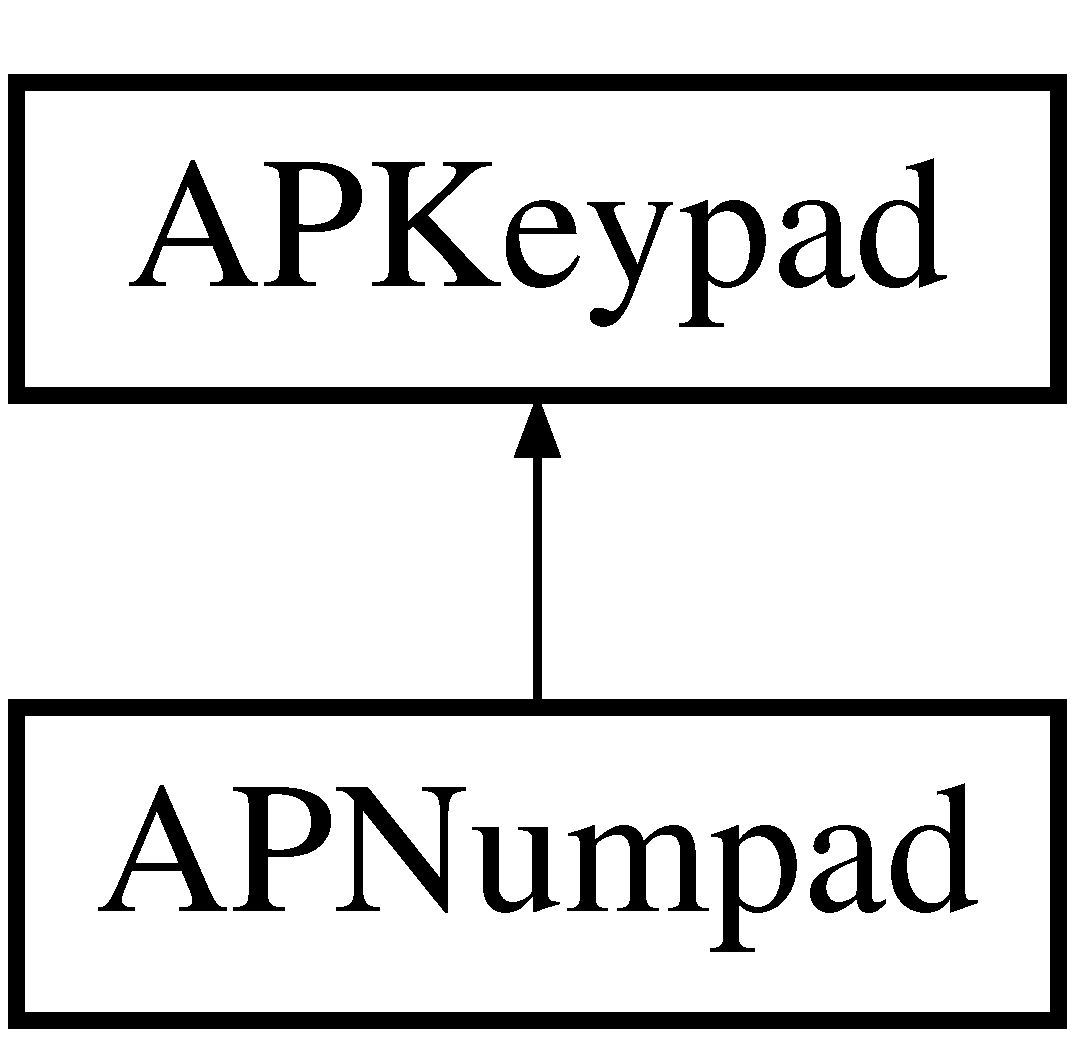
\includegraphics[height=2.000000cm]{class_a_p_keypad}
\end{center}
\end{figure}
\subsection*{Public Member Functions}
\begin{DoxyCompactItemize}
\item 
\hypertarget{class_a_p_keypad_a26e154a988dcf1b8ca5b39a2b6727af2}{void {\bfseries send\-\_\-msg} (char $\ast$msg)}\label{class_a_p_keypad_a26e154a988dcf1b8ca5b39a2b6727af2}

\item 
\hypertarget{class_a_p_keypad_ad46e3f97536b5b90556cba4de9485bab}{void {\bfseries read\-\_\-msg} (char $\ast$msg)}\label{class_a_p_keypad_ad46e3f97536b5b90556cba4de9485bab}

\end{DoxyCompactItemize}


The documentation for this class was generated from the following file\-:\begin{DoxyCompactItemize}
\item 
A\-P\-Keypad.\-h\end{DoxyCompactItemize}

\hypertarget{class_a_p_numpad}{\section{A\-P\-Numpad Class Reference}
\label{class_a_p_numpad}\index{A\-P\-Numpad@{A\-P\-Numpad}}
}
Inheritance diagram for A\-P\-Numpad\-:\begin{figure}[H]
\begin{center}
\leavevmode
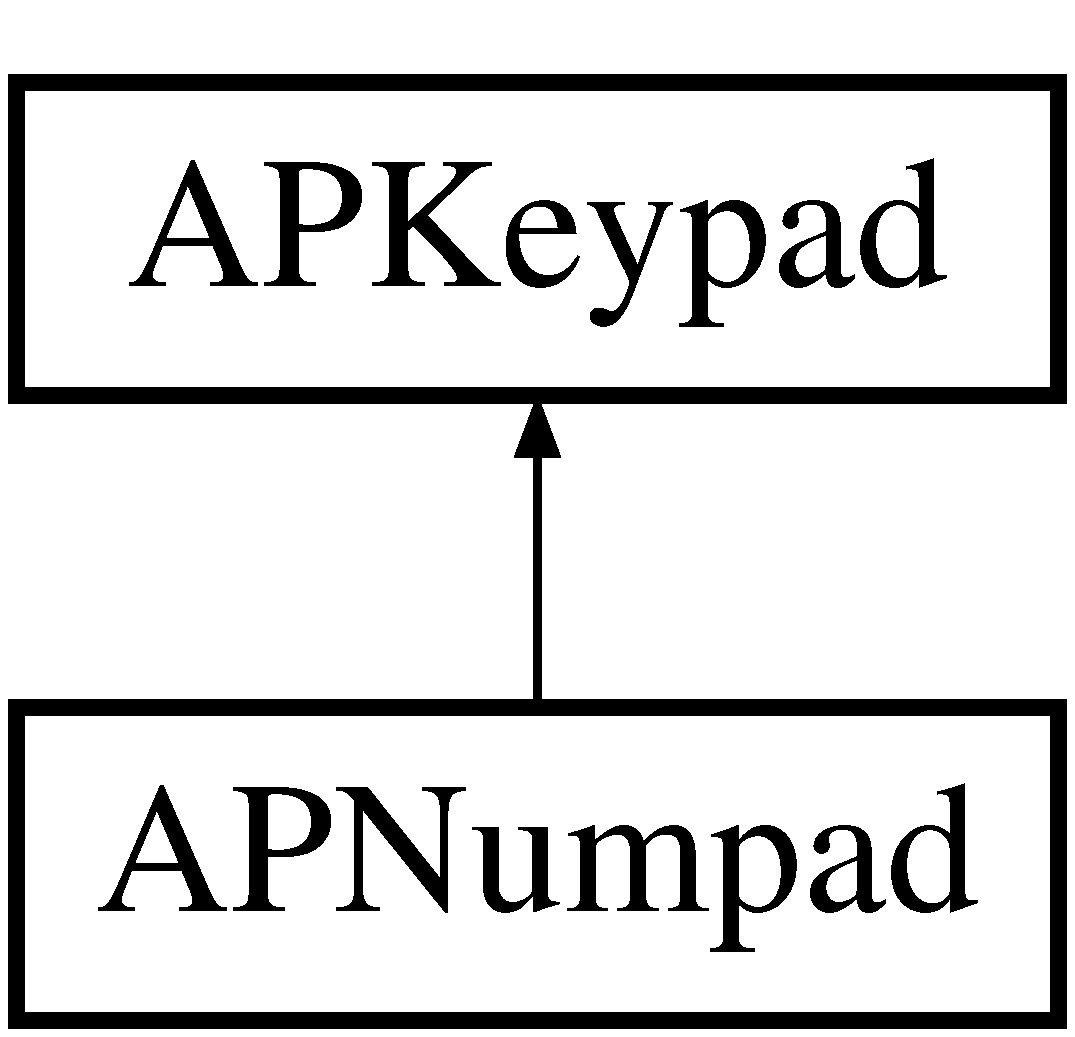
\includegraphics[height=2.000000cm]{class_a_p_numpad}
\end{center}
\end{figure}
\subsection*{Public Member Functions}
\begin{DoxyCompactItemize}
\item 
\hypertarget{class_a_p_numpad_aa499d162fb1623e00855cfade46c0b53}{void {\bfseries draw\-\_\-buttons} ()}\label{class_a_p_numpad_aa499d162fb1623e00855cfade46c0b53}

\item 
\hypertarget{class_a_p_numpad_a8c055fa67f6b7cba9f18aed4ca766b46}{char $\ast$ {\bfseries det\-\_\-touch} ()}\label{class_a_p_numpad_a8c055fa67f6b7cba9f18aed4ca766b46}

\end{DoxyCompactItemize}


The documentation for this class was generated from the following files\-:\begin{DoxyCompactItemize}
\item 
A\-P\-Keypad.\-h\item 
A\-P\-Keypad.\-cpp\end{DoxyCompactItemize}

\printindex
\end{document}
